\section{Scope and Background}
\label{sec:background}

\ignore{
\begin{enumerate}
\item abstraction refinement
\item fixpoint
\end{enumerate}
}

\begin{figure}[t]
\begin{minipage}[b]{0.49\linewidth}
\centering
\footnotesize
\begin{lstlisting}[language=Java,basicstyle=\scriptsize\ttfamily]
m(int x) {
 if(drawBernoulli(0.5) == 1) {
  if(drawBernoulli(0.5) == 1) {
   if(x <= 60)
    ...
   else
    assert false
  } else {
   if(x <= 30)
    ...
   else
    assert false
  }
 } else {
  if(x <= 55)
   ...
  else
   assert false
 }
}
\end{lstlisting}
\end{minipage}%
\begin{minipage}[b]{0.49\linewidth}
\centering
\tikzstyle{gn} = [circle, fill=gray!20, draw]
\tikzstyle{wn} = [circle, draw]
\tikzstyle{bn} = [text width=2em, text centered]
\tikzstyle{every node}=[font=\scriptsize, inner sep=0pt, minimum size=0.4cm]
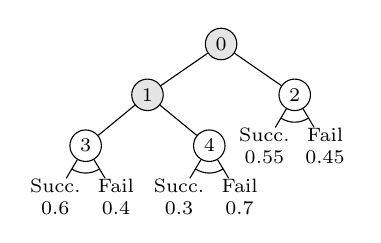
\begin{tikzpicture}[scale=0.38, level/.style={sibling distance = 15mm, level distance = 17mm}]
  \node[gn] {0}
   child{
    node[gn,xshift=-6.5mm] {1}
     child{
      node[wn,xshift=-5mm] {3}
       child{
        node[bn,xshift=-1mm] {Succ. 0.6}
        edge from parent coordinate[midway](m1)
       }
       child{
        node[bn,xshift=1mm] {Fail 0.4}
        edge from parent coordinate[midway](m2)
       }
      edge from parent
     }
     child{
      node[wn,xshift=5mm] {4}
       child{
        node[bn,xshift=-1mm] {Succ. 0.3}
        edge from parent coordinate[midway](m3)
       }
       child{
        node[bn,xshift=1mm] {Fail 0.7}
        edge from parent coordinate[midway](m4)
       }
      edge from parent
     }
   }
   child{
    node[wn,xshift=6.5mm] {2}
     child{
      node[bn,xshift=-1mm] {Succ. 0.55}
      edge from parent coordinate[midway](m5)
     }
     child{
      node[bn,xshift=1mm] {Fail 0.45}
      edge from parent coordinate[midway](m6)
     }
    edge from parent
   }
;
\draw (m1) to[bend right] (m2);
\draw (m3) to[bend right] (m4);
\draw (m5) to[bend right] (m6);
\end{tikzpicture}
\end{minipage}
\caption{Example 1}
\label{fig:example}
\end{figure}



We focus in this paper on programs that draw input variables
from given probability distributions, or equivalently that make
calls on functions returning values drawn from given distributions,
such as those provided by NetLogo which supports
uniform, normal, Poisson, exponential and gamma distributions.
\mycomment{We should pull an example from one of the later sections
back here to illustrate the idea.}

While researchers have developed analyses that consider a wide
range of program properties, here
we restrict our attention to program
properties that can be encoded as boolean predicates that
can be embedded in the program,
e.g., \texttt{assert} statements, to simplify the explanation
of how probabilities are incorporated into the analyses.
These are refered to as \textit{invariant properties} since
they are intended to hold whenever reached in all program program executions

\subsection{Programs and Program Analyses}
A program defines a set of execution \textit{traces} each of
which is a sequence of \textit{concrete states}, i.e., 
the current program counter and a map from memory locations to values.
A program \textit{satisfies} an invariant property if in all states in
all traces the predicate evaluates to true, otherwise the program
\textit{falsifies} the property.

A key concept in the program analysis frameworks we survey is
\textit{symbolic abstraction}.  A symbolic abstraction is a 
representation of a set of states.  Abstractions can be encoded
in a variety of forms, e.g., logical formula or binary
decision diagrams \cite{BDD}.  

Analyses that seek to prove the satisfaction of properties generally
define abstractions that \textit{overapproximate} the set of program
states, whereas those that seek to falsify properties generally define
abstractions that \textit{underapproximate} the set of program states.

With overapproximating analyses it is common to define an \textit{abstract
domain}, $\mathcal{A}$, 
which symbolically represents a set of concrete states which 
are said to be defined over the \textit{concrete domain}, $\mathcal{C}$.
For any reachable state of a program a pair of abstraction 
and concretization functions, 
$\alpha : \mathcal{C} \mapsto \mathcal{A}$ and  
$\gamma : \mathcal{A} \mapsto 2^\mathcal{C}$,
serve to relate the concrete and abstract domains such that 
$\forall c \in \mathcal{C} : \alpha(c) \in \mathcal{A}$ and $c \in \gamma(\alpha(c))$.
Such an abstract domain is typically partially ordered, $\sqsupseteq$,
so that 
$\forall a,a' \in \mathcal{A} :  a \sqsupseteq a' \implies \gamma(a) \supseteq \gamma(a')$.
Moreover, equiping it with a meet operator, $\sqcap$, which
computes greatest lower bounds, and a maximal
value, $\top \in \mathcal{A}$ such that 
$\forall a \in \mathcal{A} : a \sqcap \top = a$, makes the
abstract domain a meet semi-lattice.

\subsubsection{Data Flow Analysis}
Data flow analyses~\cite{Kildall} 
(and analyses built using abstract interpretation~\cite{Cousot}) perform
non-standard interpretations of program executions over an abstract domain.  
The semantics of program statements is lifted to operate
on a set of states, encoded as an element of the abstract domain,
rather than a single concrete state.  
For a program statement $\tau$,
$\tau^\#$ defines its abstract semantics such that
$\forall c, c' \in \mathcal{C} : \tau(c) = c' \implies \tau^\#(\alpha(c)) \sqsupseteq \alpha(c')$.  This implies the classic overapproximating correctness
relation for abstracted program statements:
$\tau^\# \sqsupseteq \alpha \circ \tau \circ \gamma$.

Conceptually for a program trace, $tr_i$, the sequence of 
statements, $[\tau_1,\ldots,\tau_n]$, defining the trace can
be interpreted functionally, $tr_i^\# = \tau_{n}^\# \circ \ldots \circ \tau_1^\#$,
and evaluated, $tr_i^\#(\iota)$,
to overapproximate the program states reached by the trace; 
here $\iota$ is the abstract state describing the initial program states.
Given an overapproximation of the set of traces, $T(l)$, leading to a 
program location, $l$, 
$\displaystyle\bigsqcap_j^{T(l)} tr_j^\#(\iota)$ 
defines invariant properties that hold prior to executing $l$; this
is refered to as the meet-over-paths (MOP) solution~\cite{Kildall}.

Introduce control flow graphs and talk about branch modeling.
\begin{figure}[t]
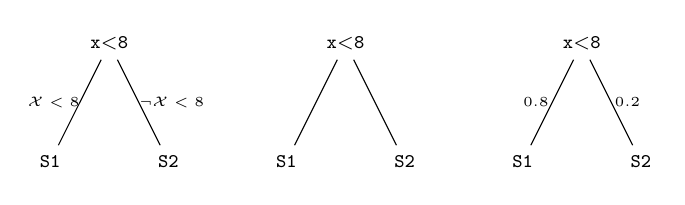
\begin{tikzpicture}[]
  \node {\texttt{x$<$8}}
     child {
        node[xshift=0mm, yshift=0mm] {\texttt{S1}}
        edge from parent
        node[left] {\tiny ${\cal X} < 8$}
     }
     child {
        node[xshift=0mm, yshift=0mm] {\texttt{S2}}
        edge from parent
        node[right] {\tiny $\neg {\cal X} < 8$}
     };
  \node[xshift=30mm] {\texttt{x$<$8}}
     child {
        node[xshift=0mm, yshift=0mm] {\texttt{S1}}
        edge from parent
     }
     child {
        node[xshift=0mm, yshift=0mm] {\texttt{S2}}
        edge from parent
     };
  \node[xshift=60mm] {\texttt{x$<$8}}
     child {
        node[xshift=0mm, yshift=0mm] {\texttt{S1}}
        edge from parent
        node[left] {\tiny $0.8$}
     }
     child {
        node[xshift=0mm, yshift=0mm] {\texttt{S2}}
        edge from parent
        node[right] {\tiny $0.2$}
     };
\end{tikzpicture}
\caption{Branch Modeling Approaches}
\label{fig:branches}
\end{figure}
Figure~\ref{fig:branches} illustrates three approaches for
modeling the program fragment: \texttt{if (x < 8) S1 else S2}.


Generating the set of traces for non-trivial programs is impractical 
and instead abstract states can be combined, via $\sqcap$, wherever
traces merge in the control flow to compute the maximum fix point (MFP)
as illustrated in Algorithm~\ref{alg-dfa}.
The algorithm stores abstract states, $a$, for each location, initializing
the first location to $\iota$, then proceeds along the control
flow relation of the program to approximate the effects of program
statements.  It removes a new location, $l$, and computes the abstract
state that approximates the post-state of executing the operation
at that location -- storing it in a temporary $t$.  Then for
all control flow successors it updates the abstract state for
that location by computing the greatest lower bound with $t$.
If that results in a new abstract state for the successor then
the successor is stored for future processing.  When the algorithm
terminates it computes for each location $l$ an approximation,
$a[l] \sqsubseteq \displaystyle\bigsqcap_j^{T(l)} tr_j^\#(\iota)$.
The nature of the MFP approximation assures that $a[l]$ defines
invariant properties that hold prior to executing statement $l$, however,
it fail to include some actual invariant properties.

Data flow analysis tools and toolkits exist for many popular 
languages~\cite{SOOT,WALA,others}
and have been used primarily for program optimization and
verifying program conformance with, implicit and explicit,
assertional specifications.

\subsubsection{Model Checking}
\mycomment{Matt: waiting for the probabilistic section to be fleshed out
to backfill this}

\begin{figure}[t]
\noindent\begin{minipage}[t]{0.32\textwidth}
\begin{algorithm}[H]
%\renewcommand{\thealgorithm}{}
\renewcommand{\algorithmicindent}{0.6em}
\floatname{algorithm}{Alg.}
\caption{{\tt dfa}$(\iota,a)$}
\label{alg-dfa}
\begin{algorithmic}
 \STATE $a[l_0] \gets \iota$
 \STATE $\forall l \not= l_0 : a[l] \gets \top$
 \STATE $w \gets \{l_0\}$
 \WHILE{$w \not= \emptyset$}
   \STATE $l \gets remove(w)$
   \STATE $t \gets {op(l)}^{\#}(a[l])$
   \FOR{$l' \in succ(l)$}
     \STATE $a[l'] \gets (o \gets a[l']) \sqcap t$
     \IF{$a[l'] \not= o$}
       \STATE $w \gets w \cup \{l'\}$
     \ENDIF
   \ENDFOR
 \ENDWHILE
 \STATE $\forall l : \x{check}(a[l],\phi)$
\end{algorithmic}
\end{algorithm}
\end{minipage}%
\hfill
\begin{minipage}[t]{0.29\textwidth}
\begin{algorithm}[H]
%\renewcommand{\thealgorithm}{}
\renewcommand{\algorithmicindent}{0.6em}
\floatname{algorithm}{Alg.}
\caption{{\tt mc}$(s,seen)$}
\label{alg-mc}
\begin{algorithmic}
 \IF{$s \not\in seen$}
   \STATE $seen \gets seen \cup \{s\}$
   \STATE $\x{check}(L(s),\phi)$
   \FOR{$s' : R(s,s')$}
     \STATE {\tt mc}$(s',seen)$
   \ENDFOR
 \ENDIF
\end{algorithmic}
\end{algorithm}
\end{minipage}%
\hfill
\begin{minipage}[t]{0.34\textwidth}
\begin{algorithm}[H]
%\renewcommand{\thealgorithm}{}
\renewcommand{\algorithmicindent}{0.6em}
\floatname{algorithm}{Alg.}
\caption{{\tt symx}$(l,m,pc)$}
\label{alg-symexe}
\begin{algorithmic}
 \WHILE{$\neg \x{branch}(l)$}
   \STATE $m \gets \x{op}(l)(m)$
   \STATE $l \gets \x{succ}(l)$
   \STATE $\x{check}(l,m,\phi)$
 \ENDWHILE

 \STATE $c \gets \x{cond}(l)$

 \IF{SAT$(pc \wedge c)$}
   \STATE {\tt symx}$(\x{succ_t}(l), m, pc \wedge c)$
 \ENDIF

 \IF{SAT$(pc \wedge \neg c)$}
   \STATE {\tt symx}$(\x{succ_f}(l), m, pc \wedge \neg c)$
 \ENDIF
\end{algorithmic}
\end{algorithm}
\end{minipage}
\end{figure}

\subsubsection{Symbolic Execution}
Like data flow analysis, symbolic execution~\cite{King1976,clarke76:system} 
performs a non-standard interpretation of program executions using 
a symbolic abstraction of program states.
Algorithm~\ref{alg-symx} sketches the symbolic execution algorithm.
The algorithm records the current program location, $l$,
and a map, $m$, that records symbolic expressions encoding the
values of program memory.  In addition a \textit{path condition}, $pc$,
accumulates symbolic expressions that encode branch constraints 
taken along a trace.  The analysis is initiated with the first
program location, $l_0$, an empty map, and $pc = true$.

Sequences of program statements are interpreted by applying the operation
at each program location, $op(l)$, to update the map.  
An operation that reads from an input generates a fresh symbolic
variable which is unconstrained.  
When a branching statement is encountered the symbolic expression encoding
the branch condition is computed, $c$, and a check is performed
to determine whether the current trace, encoded by $pc$, can be
extended with $c$ or its negation.  
This is achieved by formulating the constraints
as a satisfiability query -- if the formula encoding branch constraints
is satisfiable then it there must exist an input that will follow the trace.
The trace is extended, recursively, following the feasible branch outcomes
in a depth-first manner.

While this algorithm is capable of computing an \textit{exact} symbolic
approximation of the set of program states on a trace reaching $l$, in
practice symbolic execution computes an underapproximation.
Programs with looping behavior that is determined by input values 
may result in an infinite symbolic execution tree. 
For this reason, symbolic execution is
typically run with a (user-specified) bound on the search depth, thus
some paths may be unexplored.   Moreover, there may be path constraints
for which efficient satisfiable checking is not possible.  Variants of
symbolic execution~\cite{godefroid05:dart,Cute,BitBlaze} 
address this by replacing problematic $pc$ constraints with equality
constraints based on values collected by executing the program along the trace.

Symbolic execution tools and toolkits exist for many popular 
languages~\cite{SPF,godefroid05:dart,tillman-halleux-tap2008,Klee}
and have been used primarily for test generation and fault detection.

\subsection{Probabilities and Probabilistic Models}

The probability of an event $e$ is written $Pr(e)$.

Define and explain the following
\begin{itemize}
\item basic definitions that you think we need
\item discrete time Markov chain
\item discrete time Markov decision process
\end{itemize}

